\section{S3}

\begin{frame}[allowframebreaks]
	\frametitle{Amazon S3}
	\begin{itemize}
		\item Amazon Simple Store Service
		\item Armazena objetos:
			\begin{itemize}
				\item Dados
				\item Metadados (Pares chave-valor)
			\end{itemize}
		\item Cada objeto tem um identificador único (Global)
		\item Pode habilitar versionamento
		\item Objetos não são deletados (são marcados como deletado)
	\end{itemize}
	\begin{figure}[htpb]
	\begin{center}
	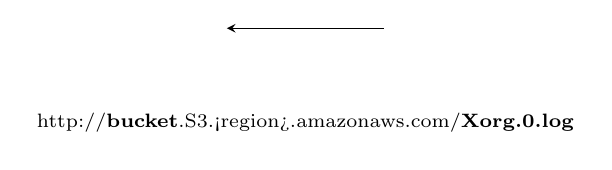
\begin{tikzpicture}[scale=1, transform shape]
		\node at (0,-1.5) {\scriptsize http://\textbf{bucket}.S3.<region>.amazonaws.com/\textbf{Xorg.0.log}};
		\bucket{-1.5}{0}{0.3}{\tiny bucket}
		\file{1.5}{-0.3}{0.3}{\tiny log/Xorg.0.log}
		\draw[stealth-] (-1,-0.3) -- (1,-0.3);
	\end{tikzpicture}
	\end{center}
	\caption{Endereço S3}
	\end{figure}
	\framebreak
	\begin{itemize}
		\item Storage classes
			\begin{itemize}
				\item S3 Standard
				\item S3 Intelligent - Tiering
				\item S3 Standard - IA
				\item S3 One zone - IA
				\item S3 Glacier Instant Retrieval
				\item S3 Glacier Flexible Retrieval
				\item S3 Glacier Deep Archive
			\end{itemize}
	\end{itemize}
\end{frame}

\begin{frame}
	\frametitle{S3 Features}
	\begin{itemize}
	\begin{small}
		\item \textbf{S3 Storage class analysis}: Descobrir padrões de acesso
		\item \textbf{S3 Lifecycle policy}: Quando os dados devem ser transferidos para outro tipo de storage class
		\item \textbf{S3 Cross-Region Replication (CRR)}: Replicar buckets entre diferentes regiões
		\item \textbf{S3 Same Regnio Replication}: Replicar buckets na mesma região
		\item \textbf{S3 Object Lock}: Não permite que o bucket seja apagado
		\item \textbf{S3 Inventory}: Lista de objetos e status da criptografia
		\item \textbf{S3 Batch operations}: Copiar objetos de buckets, colocar tags, modificar acesso, etc\dots
		\item \textbf{S3 Select}: Aumenta a performace da query e reduz os custos
	\end{small}
	\end{itemize}
\end{frame}

\begin{frame}
	\frametitle{S3 Access Management}
	\begin{itemize}
		\item Buckets são privados por padrão
		\begin{itemize}
			\item O dono do recurso da acesso para os outros 
		\end{itemize}
		\item Resource-based policies
			\begin{itemize}
				\item Bucket policies: escrito em Json e permite/bloqueia usuários em determinado bucket
				\item Access Control Lists (ACLs) usa xml e define quem tem permissão para usar o bucket
			\end{itemize}
		\item User policies (IAM)
	\end{itemize}
\end{frame}
